\documentclass[a4paper,12pt]{article}

\usepackage[slovene]{babel}
\usepackage[utf8]{inputenc}
\usepackage[T1]{fontenc}
\usepackage{lmodern}
\usepackage{amsmath}
\usepackage{amssymb}
\usepackage{amsthm}
\usepackage{amsfonts}
\usepackage{mathtools}
\usepackage{enumitem}
\usepackage[table,xcdraw]{xcolor}


\begin{document}

\begin{titlepage}
    \centering
    \vfill
    \vfill
    \textbf{\large{POROČILO SEMINARSKE NALOGE}}
    \vfill
    \textbf{\Huge{STATISTIKA}}
    \vfill\vfill\vfill\vfill\vfill
    \textsc{\Large{Sara Bizjak}}
    \vfill\vfill
    \textsc{\large{Univerza v Ljubljani}}
    
    \textsc{\large{Fakulteta za matematiko in fiziko}}
    
    \textsc{\large{Oddelek za matematiko}}
    \vfill\vfill
        
    \large{JULIJ 2020}
    
\end{titlepage}

%%%

\newpage

%%%%%%%%%%%%%%%%%%%%%%%%%%%%%%%%%%%%%%%%%%%%%%%%%%%%%%%%%%%%%%

\noindent
\textsc{\large{1. NALOGA}}
\\
\\
Podatki so vzeti iz datoteke \texttt{Kibergard}, kjer se nahajajo informacije o 43.886 družinah, ki stanujejo v mestu Kibergard. Za vsako družino so zabeleženi naslednji podatki:
\begin{itemize}
    \item Tip družine (od 1 do 3)
    \item Število članov družine
    \item Število otrok v družini
    \item Skupni dohodek družine
    \item Mestna četrt, v kateri stanuje družina (od 1 do 4)
    \item Stopnja izobrazbe in vodje gospodinjstva (od 31 do 46: opisi v datoteki z navodili)
\end{itemize}

\noindent
Nalogo sem reševala s pomočjo programa R. Koda, uporabljena za generiranje enostavnih slučajnih vzorcev in izračune, je priložena na koncu poročila pod naslovom \textit{Dodatek A}, dostopna pa je tudi v priloženi datoteki \textit{naloga1.R}. 
\\

%%%%%%%%%%%%%%%%%%%%%%%%%%%%%%%%

\noindent
\textsc{\underline{Primer a}}
\\
Vzamemo enostavni slučajni vzorec 200 družin in na njegovi podlagi ocenimo delež družin v Kibergardu, v katerih vodja gospodinjstva nima srednješolske izobrazbe (niti poklicne niti splošne mature).
Opisan delež znaša $p = 0.195$.
\\

%%%%%%%%%%%%%%%%%%%%%%%%%%%%%%%%

\noindent
\textsc{\underline{Primer b}}
\\
Ocenimo standardno napako in postavimo 95\% interval zaupanja.

\noindent
Standardno napako za delež izračunamo po formuli (na strani 210 v knjigi \textit{John A. Rice: Mathematical Statistics and Data Analysis}):
$$ \hat{se}(p) = \sqrt{ \frac{p \cdot (1-p)}{n} \cdot \left(1 - \frac{n - 1}{N - 1} \right)}, $$
kjer so $p = 0.195$, \ $n = 200$, \ $N = 43.886$. 
\\
Dobimo rezultat $\hat{se}(p) = 0.02795203$.
\\
Interval zaupanja je enak: $[0.140215, 0.249785]$.
\\

%%%%%%%%%%%%%%%%%%%%%%%%%%%%%%%%

\noindent
\textsc{\underline{Primer c}}
\\
Vzorčni delež in ocenjeno standardno napako primerjamo s populacijskim deležem in pravo standardno napako. 
\\
\begin{itemize}
\item Vzorčni delež: $0.195$ 
\item Populacijski delež: $0.2115025$ 
\item Razlika obeh deležev: $0.01650253$
\item Ocenjena standardna napaka (iz vzorca): $0,02802185$
\item Prava standardna napaka (iz celotne populacije):  $0.02881085$
\item Razlika med ocenjeno in pravo standardno napako: $0.0008588181$
\end{itemize}
Ker velja $0.2115025 \in [0.140215, 0.249785]$, interval zaupanja pokrije populacijski delež.
\\

%%%%%%%%%%%%%%%%%%%%%%%%%%%%%%%%

\noindent
\textsc{\underline{Primer d}}
\\
Poleg vzorca iz točke a) vzamemo še $99$ enostavnih slučajnih vzorcev po 200 družin in prav tako za vsakega določimo $95 \%$ interval zaupanja. Intervale zaupanja prikažemo na grafu in ugotovimo, koliko jih pokrije populacijski delež.
\begin{figure}[ht!]
    \centering
    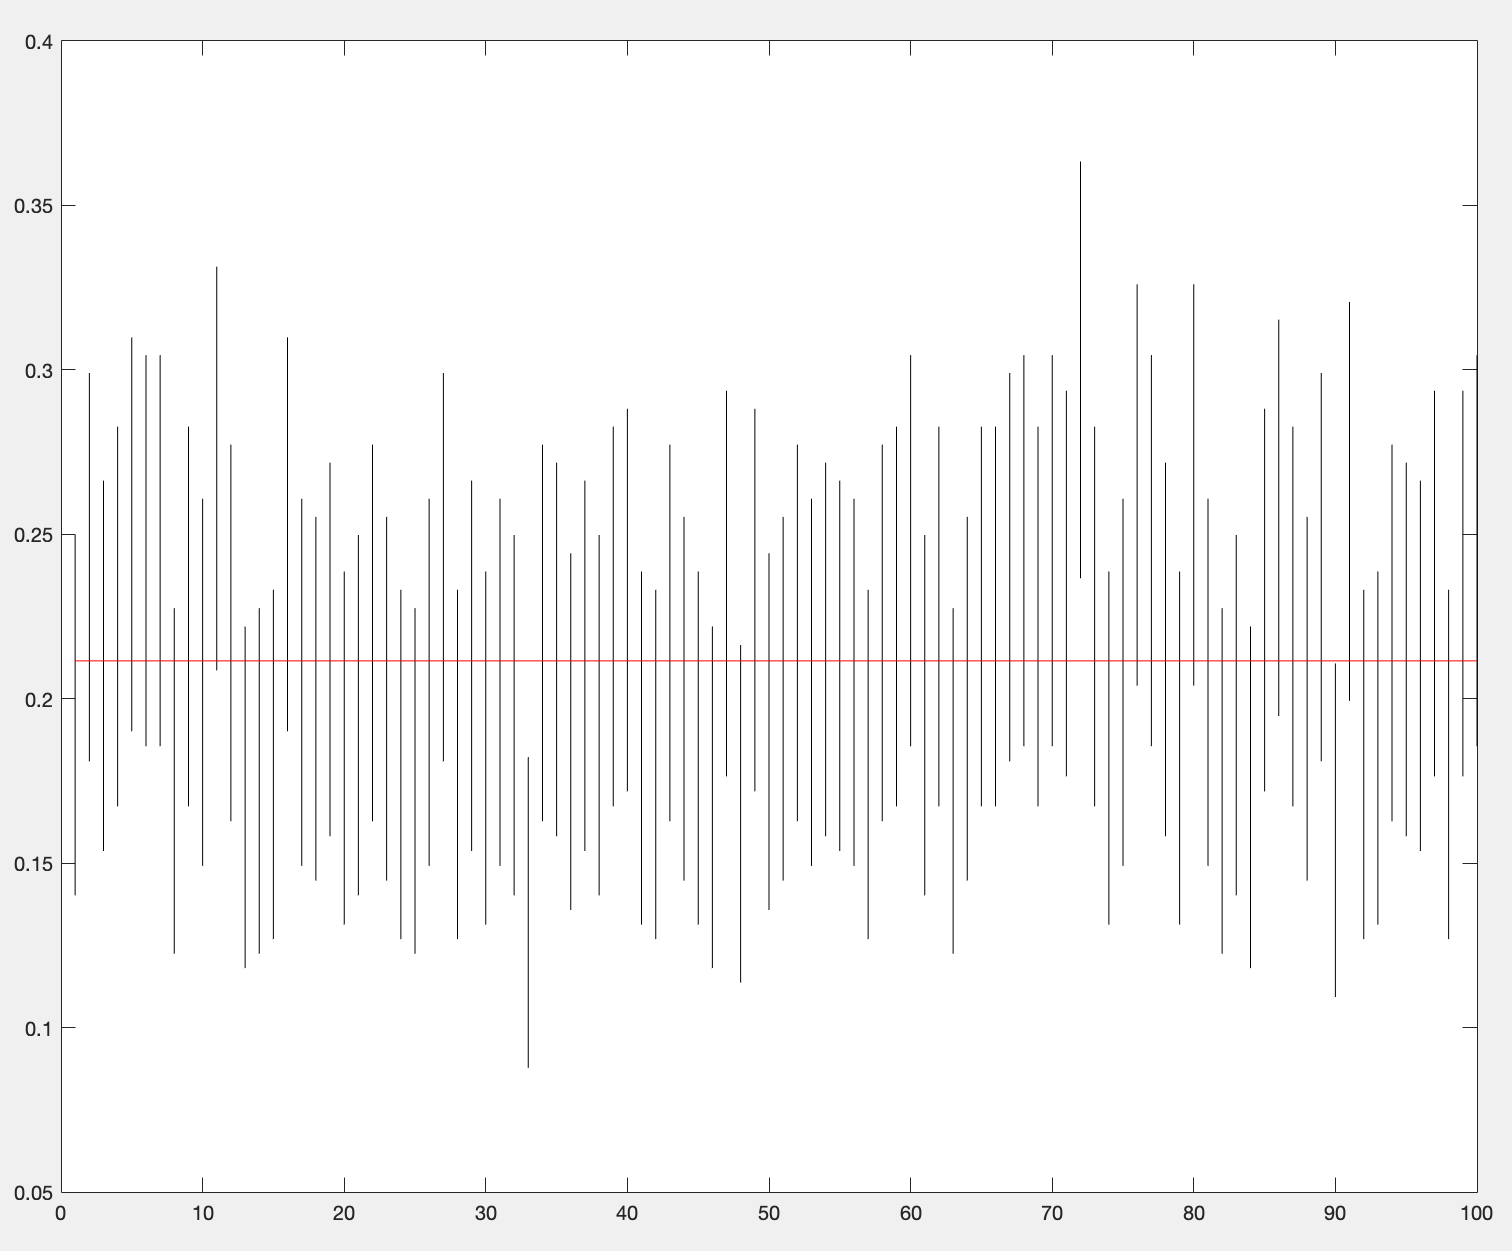
\includegraphics[width=120mm]{CI_200.png}
    \caption{Intervali zaupanja za 100 slučajnih vzorcev velikosti 200.}
\end{figure}

\noindent
Izmed 100 intervalov zaupanja jih 97 pokrije populacijski delež. To vidimo tudi na grafu, kjer rdeča črta označuje populacijski delež.
\\
%%%%%%%%%%%%%%%%%%%%%%%%%%%%%%%%

\noindent
\textsc{\underline{Primer e}}
\\
Standardni odklon vzorčnih deležev za $100$ prej dobljenih vzorcev je enak $0.00140308$. Prava standardna napaka za vzorec velikosti $200$ pa je $0.02881085$.
Razlikujeta se za $0.02740777$.
\\

%%%%%%%%%%%%%%%%%%%%%%%%%%%%%%%%

\noindent
\textsc{\underline{Primer f}}
\\
Vzamemo 100 slučajnih vzorcev po 800 družin. Za vsakega določimo $95 \%$ interval zaupanja in intervale prikažemo na grafu in ugotovimo, koliko jih pokrije populacijski delež. 
\begin{figure}[ht!]
    \centering
    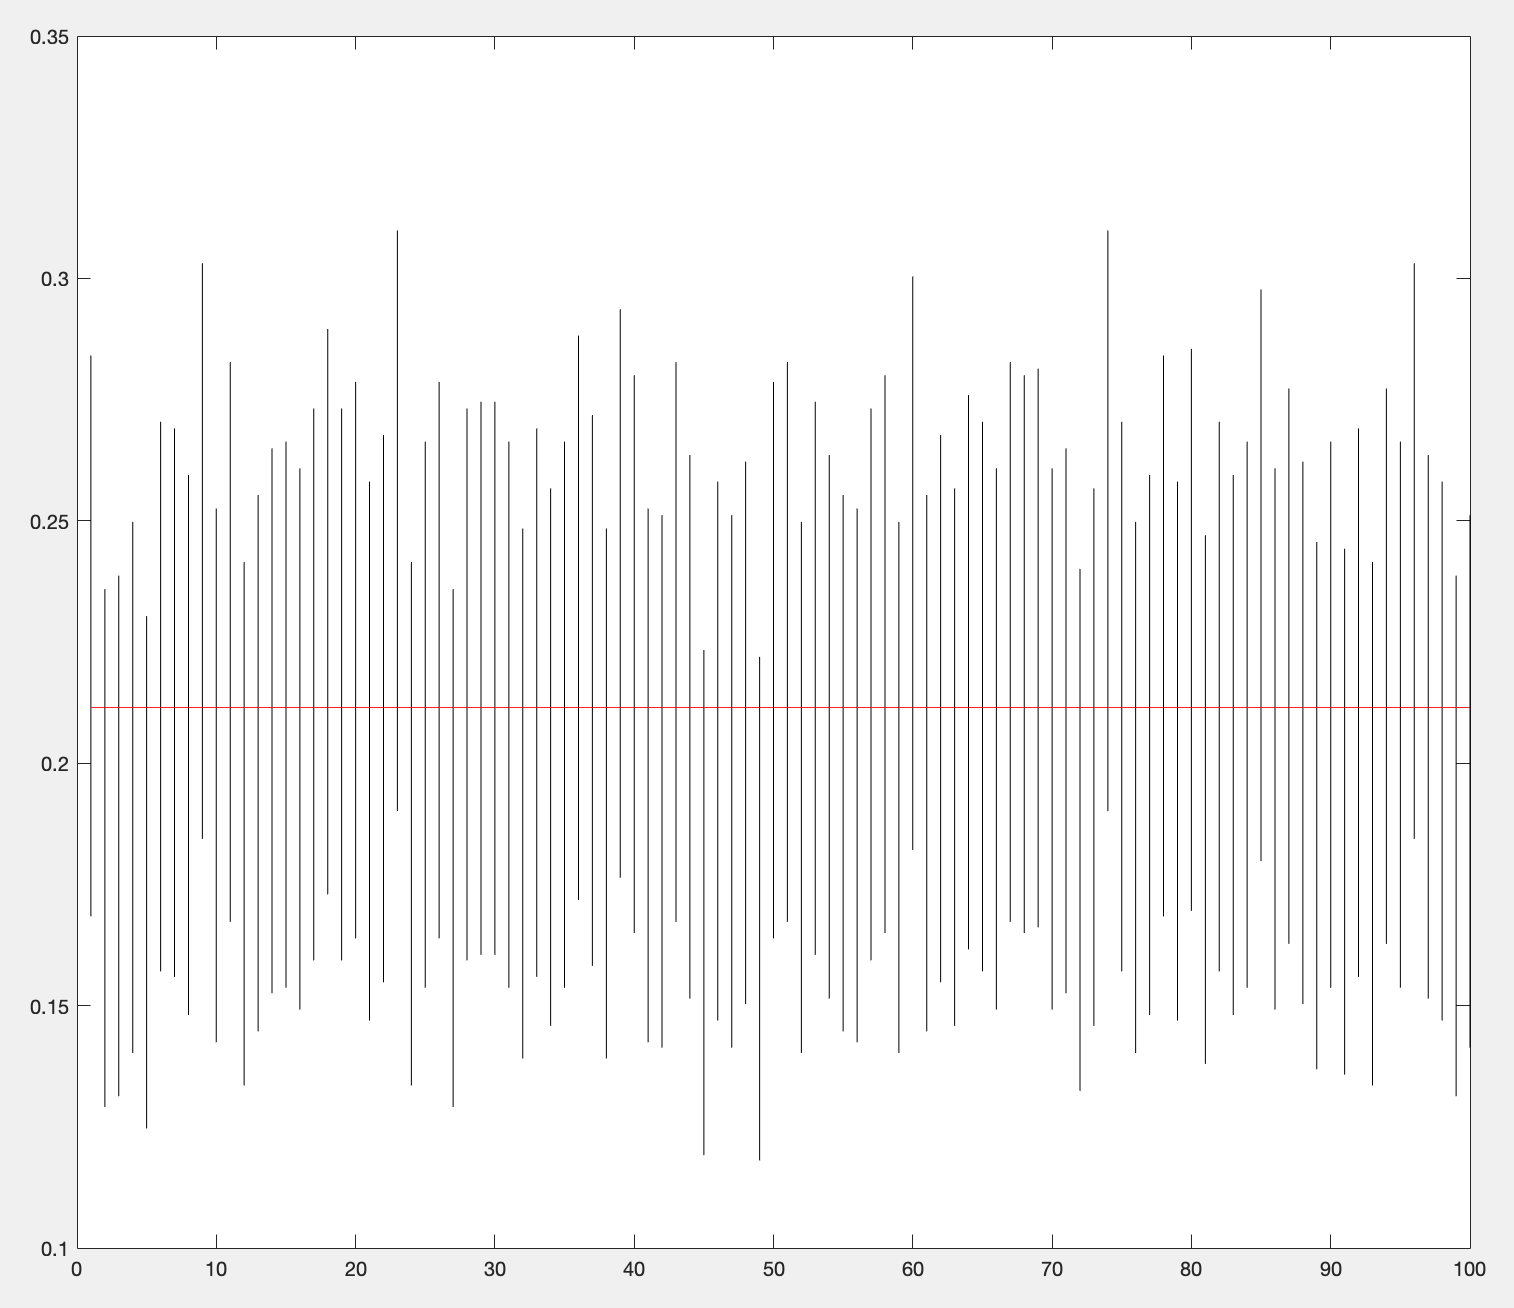
\includegraphics[width=120mm]{CI_800.png}
    \caption{Intervali zaupanja za 100 slučajnih vzorcev velikosti 800.}
\end{figure}

\noindent
Izmed 100 intervalov zaupanja vzorcev po 800 jih vseh 100 pokrije poulacijski delež. To vidimo tudi na grafu, kjer rdeča črta označuje populacijski delež.
\\
Standardni odklon vzorčnih deležev za $100$ dobljenih vzorcev velikosti $800$ je enak $0.0008074025$. Prava standardna napaka za vzorec velikosti $800$ pa je $0.01430616$.
Razlikujeta se za $0.01349875$.
\\
\\
V primeru, ko smo vzeli $100$ vzorcev velikosti $800$, smo dobili boljše rezultate kot pri izbiri $100$ vzorcev velikosti $200$. 
Praviloma lahko z izbiro večjega vzorca dobimo boljše napovedi, vendar moramo pri tem paziti še na dober vzorčni načrt. Vzorčni načrt je v naprej predpisan postopek izbiranja vzorca iz vnaprej določene in natančno opredeljene populacija. 
Način vzorčenja bistveno vpliva na zanesljivost ocen. Če je izbira enot iz populacije naključna, potem takemu vzorčenju pravimo verjetnostno vzorčenje. Z vpeljavo naključnosti se najboljse izognemo pristranskosti.
Primer slabega vzorčnega načrta in posledično napačnih napovedi je napoved izida volitev v ZDA leta 1936. 
\\

%%%%%%%%%%%%%%%%%%%%%%%%%%%%%%%%%%%%%%%%%%%%%%%%%%%%%%%%%%%%%%

\noindent
\textsc{\large{2. NALOGA}}
\\
\\
Sklepi in izpeljave, ki jih bom uporabila pri vseh podnalogah, sledijo dokazu izreka v knjigi \textit{John A. Rice: Mathematical Statistics and Data Analysis} (stran $232$, $233$).
\\
Naredimo raziskavo na populaciji, ki ima $K$ stratumov z velikostmi $N_1, N_2, \ldots, N_K$. Denimo, da lahko izberemo vzorec velikosti $n$.
\\

\noindent
\textsc{\underline{Primer a}}
\\
Denimo, da so stroški raziskave enaki $C = C_0 + n C_1$, kjer je $n$ število enot v vzorcu ($C_0$ je začetni stršek, $C_1$ pa je nadaljnji strošek na enoto). Pri danih sredstvih za raziskavo v višini $C$ poiščemo velikosti podvzorcev $n_1, n_2, \ldots, n_K$, pri katerih je varianca standardne cenilke populacijskega povprečja minimalna.
\\
Če imamo stratume velikosti $N_1, N_2, \ldots, N_K$, se moramo odločiti, kako velike vzorce bomo izbrali iz posameznih stratumov. Izbiramo tako, da bo varianca cenilke $\overline{X}$ čim manjša. 
Poiščemo torej take $n_1, n_2, \ldots, n_K$, kjer $n = n_1 + n_2 + \ldots + n_K$, da bo $$ \text{var}(\overline{X}) = \sum_{k = 1}^{K} W_k ^ 2 \left( \frac{ \sigma_k^2}{n_k} \right) \left( \frac{N_k - n_k}{N_k - 1} \right) $$
čim manjša.
Ker so v večini praktičnih situacij korekturni faktorji $\frac{N_k - n_k}{N_k - 1} \approx 1$, jih lahko zanemarimo. Rešujemo torej problem vezanega ekstrema:
$$ f(n_1, n_2, \ldots, n_K) = \sum_{k = 1}^{K} \frac{\sigma_k^2}{n_k} W_k^2 $$
$$ \text{z vezjo} \  C = C_0 + nC_1.$$
Sestavimo Lagrangeovo funkcijo:
$$ F(n_1, n_2, \ldots, n_K, \lambda) = f(n_1, n_2, \ldots, n_K) + \lambda (C_0 + \sum_{k = 1}^{K} n_k C_1 - C). $$
Zapišemo parcialne odvode funkcije $F$ in jih enačimo z $0$.
$$ \frac{ \partial F}{\partial n_i} = - \frac{ \sigma_i^2}{n_i^2} \  W_i^2 + \lambda \ C_1 = 0 \ \ \ \text{za} \ i = 1, 2, \ldots, K. $$
Izrazimo $n_i$ in dobimo sistem enačb
\begin{align}\label{en:nk}
n_i = \frac{W_i \sigma_i}{ \sqrt{ \lambda \ C_1}}
\end{align}
Da določimo $\lambda$, naredimo vsoto enačbe (\ref{en:nk}) po $i$, $i = 1, 2, \ldots, K.$
$$ n = \frac{1}{\sqrt{\lambda \ C_1}} \sum_{k = 1}^{K} W_k \sigma_k $$
\begin{align}\label{en:lambda}
\Rightarrow \sqrt{\lambda} = \frac{\sum_{k = 1}^{K} W_k \sigma_k}{n \sqrt{C_1}}
\end{align}
Če združimo (\ref{en:nk}) in (\ref{en:lambda}), dobimo:

$$ n_i = n \ \frac{W_i \sigma_i}{\sum_{k = 1}^{K} W_k \sigma_k}. $$
Rezultat je enak, kot če bi iskali minimalno varianco brez danega začetnega pogoja -- ni pomembno, kakšne $n_1, n_2, \ldots, n_K$ izberemo. Stroški raziskave $C$ bodo vedno enaki, ker je cena $C_1$ vedno enaka.
\\

\noindent
\textsc{\underline{Primer b}}
\\
Sedaj se lahko stroški opažanja spreminjajo od stratuma do strauma. Če je $n_k$ število enot iz $k-$tega stratuma, ki so zajete v vzorec, naj bodo stroški raziskave enaki:
$$ C = C_0 + \sum_{k = 1}^{K}n_k C_k. $$
Pri danih sredstvih za raziskavo v višini $C$ poiščemo tiste velikosti podvzorcev, pri katerih je varianca cenilke populacijskega povprečja minimalna.
\\
Rešujemo podoben primer kot prej, le da sedaj nimamo več fiksne $C_1$, ampak se spreminja z vsakim stratumom. 
Z enakim razmislekom kot prej sestavimo Lagrangeovo funkcijo:
$$ F(n_1, n_2, \ldots, n_K, \lambda) = f(n_1, n_2, \ldots, n_K) + \lambda (C_0 + \sum_{k = 1}^{K} n_k C_k - C). $$
Zapišemo parcialne odvode funkcije $F$ in jih enačimo z $0$.
$$ \frac{ \partial F}{\partial n_i} = - \frac{ \sigma_i^2}{n_i^2} \  W_i^2 + \lambda \ C_i = 0 \ \ \ \text{za} \ i = 1, 2, \ldots, K.  $$
Izrazimo $n_i$ in dobimo sistem enačb
\begin{align}\label{en:nkb}
n_i = \frac{W_i \sigma_i}{ \sqrt{ \lambda \ C_i}}
\end{align}
Da določimo $\lambda$, naredimo vsoto enačbe (\ref{en:nkb}) po $i$, $i = 1, 2, \ldots, K.$
$$ n = \frac{1}{\sqrt{\lambda}} \sum_{k = 1}^{K} \frac{W_k \sigma_k}{\sqrt{C_k}} $$
\begin{align}\label{en:lambdab}
\Rightarrow \sqrt{\lambda} = \frac{1}{n} \sum_{k = 1}^{K} \frac{W_k \sigma_k}{\sqrt{C_k}}
\end{align}
Če združimo (\ref{en:nkb}) in (\ref{en:lambdab}), dobimo:

$$ n_i = \frac{n}{\sqrt{C_i}} \ \frac{W_i \sigma_i}{\sum_{k = 1}^{K} \frac{W_k \sigma_k}{\sqrt{C_k}}}. $$
\\

\noindent
\textsc{\underline{Primer c}}
\\
Naj se stroški raziskave izražajo na enak način kot v prejšnji točki, predpisano pa imamo natančnost raziskave, torej varianco cenilke. Poiščemo tiste vrednosti podvzorcev, pri katerih bodo stroški najmanjši.
\\
Želimo torej minimizirati stroške pri pogoju $ \text{var}(\overline{X}) = \sum_{k = 1}^{K} \frac{W_k^2 \sigma_k^2}{n_k}.$ Označimo $\text{var}(\overline{X}) = V,$ kjer je $V$ predpisana vrednost.
\\
Rešujemo torej vezani ekstrem za funkcijo:
$$ f (n_1, n_2, \ldots, n_K) = C_0 + \sum_{k = 1}^{K} n_k C_k $$
$$ \text{z vezjo} \ \sum_{k = 1}^{K} \frac{W_k^2 \sigma_k^2}{n_k} - V. $$
Sestavimo Lagrangeovo funkcijo:
$$ F (n_1, n_2, \ldots, n_K, \lambda) = C_0 + \sum_{k = 1}^{K} n_k C_k  + \lambda \left( \sum_{k = 1}^{K} \frac{W_k^2 \sigma_k^2}{n_k} - V \right)$$
Zapišemo parcialne odvode funkcije $F$ in jih enačimo z $0$.
$$ \frac{ \partial F}{\partial n_i} = C_i - \lambda \ \frac{W_i^2 \sigma_i^2}{n_i^2} = 0 \ \ \ \text{za} \ i = 1, 2, \ldots, K.  $$
Izrazimo $n_i$ in dobimo sistem enačb
\begin{align}\label{en:nkc}
n_i = \sqrt{\frac{\lambda}{C_i}} \ W_i \sigma_i
\end{align}
Da določimo $\lambda$, naredimo vsoto enačbe (\ref{en:nkc}) po $i$, $i = 1, 2, \ldots, K.$
$$ n = \sqrt{\lambda} \ \sum_{k = 1}^{K} \frac{W_k \sigma_k}{\sqrt{C_k}} $$
\begin{align}\label{en:lambdac}
\Rightarrow \sqrt{\lambda} = \frac{n}{\sum_{k = 1}^{K} \frac{W_k \sigma_k}{\sqrt{C_k}}}
\end{align}
Če združimo (\ref{en:nkc}) in (\ref{en:lambdac}), dobimo:

$$ n_i = \frac{n}{\sqrt{C_i}} \ \frac{W_i \sigma_i}{\sum_{k = 1}^{K} \frac{W_k \sigma_k}{\sqrt{C_k}}}. $$
\\

%%%%%%%%%%%%%%%%%%%%%%%%%%%%%%%%%%%%%%%%%%%%%%%%%%%%%%%%%%%%%%

\noindent
\textsc{\large{3. NALOGA}}
\\
\\
Opazimo $n$ neodvisnih realizacij zvezne porazdelitve z gostoto:
\begin{displaymath}
    f(x \ | \ \alpha) = \left\{ \begin{array}{ll}
     \frac{\Gamma(2 \alpha)}{(\Gamma (\alpha))^2} \left[ x(1 - x) \right]^{\alpha - 1} & \textrm{; \ $0 < x < 1$}\\
     0 & \textrm{; \ sicer,} \\
    \end{array} \right. 
\end{displaymath}
kjer je $\alpha > 0$ neznam parameter. Če je $X$ slučajna spremenljivka s to gostoto, se da izračunati:
$$ \text{E}(X) = \frac{1}{2} \ , \ \ \ \ \ \text{var}(X) = \frac{1}{4(2 \alpha + 1)}. $$
\\

\noindent
\textsc{\underline{Primer a}}
\\
Določimo obliko porazdelitve v odvisnosti od $\alpha$. 
\begin{figure}[ht!]
    \centering
    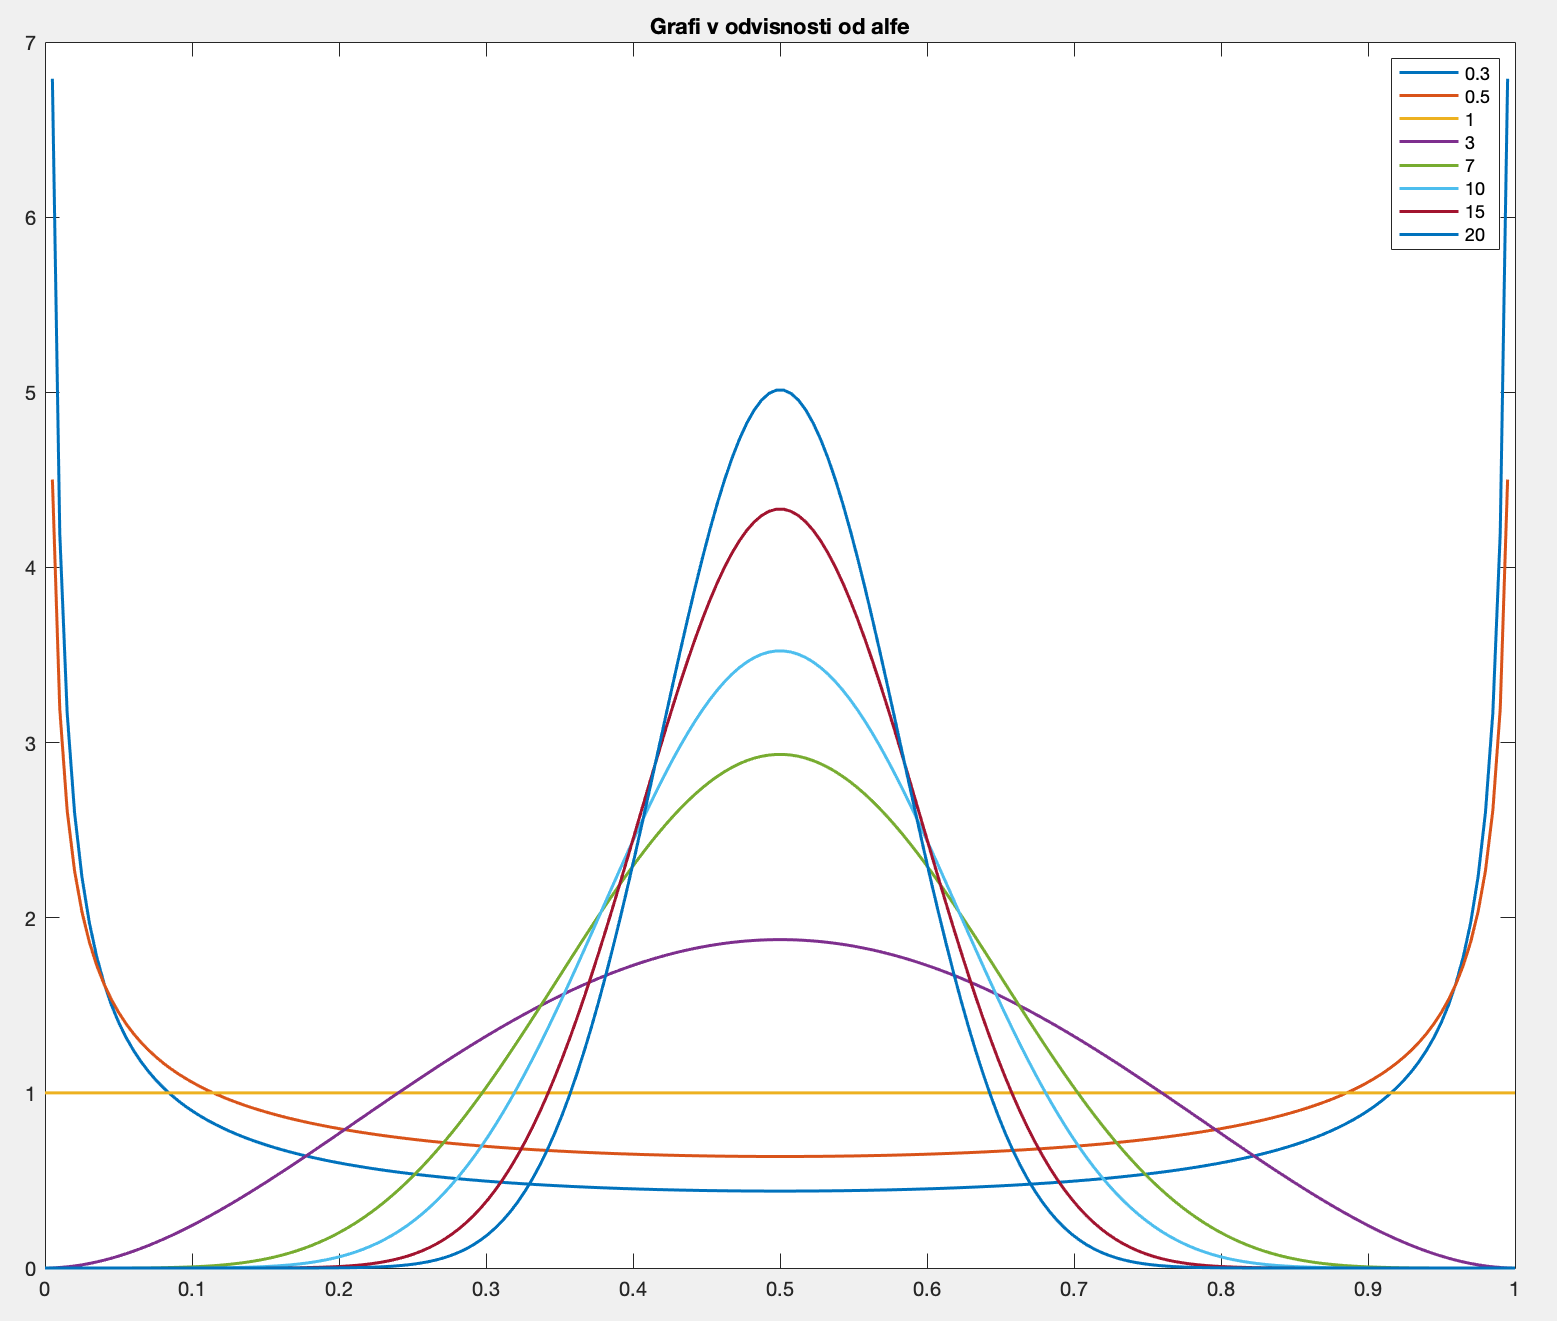
\includegraphics[width=90mm]{grafi.png}
    \caption{Grafi podane funkcije za različne $\alpha$.}
\end{figure}
Vidimo, da je funkcija $f(x \ | \ \alpha)$ simetrična glede na $x = \frac{1}{2}$ in ima v tej točki ekstrem ne glede na vrednost $\alpha$. Opazimo tudi, da je funkcija za $\alpha = 1$ kar vodoravna premica. Za $\alpha < 1$ je funkcija konveksna, za $\alpha > 1$ pa konkavna. 
Z večanjem $\alpha$ postaja funkcija vse bolj strma in \textit{"ožja"}.
\\

\noindent
\textsc{\underline{Primer b}}
\\
Ocenimo $\alpha$ po metodi momentov.
\\
Iz podane pričakovane vrednosti in variance lahko izračunamo vrednosti prvega in drugega momenta.
$$ \text{E}(X) = \frac{1}{n} \sum_{i = 1}^{n} X_i = \frac{1}{2}, $$
$$ \text{E}(X^2) = \frac{1}{n} \sum_{i = 1}^{n} X_i^2 = \text{var}(X) + \text{E}(X)^2 = \frac{1}{4(2 \alpha + 1)} + \frac{1}{4}. $$

Iz enačbe drugega momenta izrazimo $\alpha$.
\begin{align*}
    \frac{1}{4(2 \alpha + 1)} + \frac{1}{4} &= \frac{1}{n} \sum_{i = 1}^{n} X_i^2 
    \\
    \frac{1}{4(2 \alpha + 1)} &= \frac{1}{n} \sum_{i = 1}^{n} X_i^2 - \frac{1}{4} 
    \\
    \frac{1}{2 \alpha + 1} &= \frac{4}{n} \sum_{i = 1}^{n} X_i^2 - 1 
    \\
    2 \alpha + 1 &= \frac{1}{\frac{4}{n} \sum_{i = 1}^{n} X_i^2 - 1}
    \\
    \Rightarrow \hat{\alpha} &= \frac{1}{2} \left( \frac{1}{\frac{4}{n} \sum_{i = 1}^{n} X_i^2 - 1} - 1 \right).
\end{align*}

\noindent
\textsc{\underline{Primer c}}
\\
Poiščemo enačbo, ki določa cenilko po metodi največjega verjetja. Pogledamo, kdaj ta cenilka obstaja.
$$ L_1 (\alpha \ | \ x_1) = \frac{\Gamma (2 \alpha)}{\Gamma (\alpha)^2} \ x_1^{\alpha - 1} (1 - x_1)^{\alpha - 1} $$
$$ l_1 (\alpha \ | \ x_1) = \text{ln}(\text{L}_1 (\alpha | x_1)) $$
$$ \Rightarrow l_1 (\alpha \ | \ x_1) = \text{ln}(\Gamma (2 \alpha)) - 2 \text{ln} (\Gamma (\alpha)) + (\alpha - 1) \text{ln}(x_1) + (\alpha - 1) \text{ln}(x_1 - 1) $$
\\
$$ l (\alpha \ | \ x) = \sum_{i = 1}^{n} \text{l}_1 (\alpha | x_1) $$
$$ \Rightarrow l (\alpha \ | \ x) = n \cdot \text{ln}(\Gamma (2 \alpha)) - 2 n \cdot \text{ln}(\Gamma (\alpha)) + (\alpha - 1) \sum_{i = 1}^{n} \text{ln}(x_i) + (\alpha - 1) \sum_{i = 1}^{n} \text{ln} (x_i - 1)$$
\\
Funkcijo $ l (\alpha \ | \ x) $ odvajamo po $\alpha$.
$$ \frac{\partial l}{\partial \alpha} = n \cdot \frac{1}{\Gamma (2 \alpha)} \cdot 2 \Gamma' (2 \alpha) - 2n \cdot \frac{1}{\Gamma (\alpha)} \cdot \Gamma' (\alpha) + \sum_{i = 1}^{n} \text{ln}(x_i) + \sum_{i = 1}^{n} \text{ln}(x_i - 1)$$
Cenilka bo obstaja natanko tedaj, ko bo imela enačba
 $$ \frac{1}{\Gamma (2 \alpha)} \cdot \Gamma' (2 \alpha) - \frac{1}{\Gamma (\alpha)} \cdot \Gamma' (\alpha) = \frac{1}{2n} \ \sum_{i = 1}^{n} \text{ln} \left( \frac{1}{x_i(x_i - 1)} \right) $$
rešitev.

\noindent
\textsc{\underline{Primer d}}
\\
Poiščemo asimptotično varianco cenilke po metodi največjega verjetja.
\\
Za asimptotično varianco bomo potrebovali Fischerjevo informacijo za cenilko, saj velja 
$$\text{var}(\hat{\alpha}) \approx \frac{1}{n \cdot I_1(\hat{\alpha})}, $$
kjer (iz predavanj) 
\begin{align}\label{en:fish}
    I_1(\hat{\alpha}) &= - \text{E} \left[ \frac{ \partial^2 \ l_1(\alpha \ | \ x_1)}{\partial \alpha^2} \right]
\end{align}
V $\frac{\partial l}{\partial \alpha}$ vstavimo $n = 1$ in izračunamo še drugi odvod. Dobimo:
$$ \frac{\partial^2 l_1}{\partial \alpha^2} = \frac{4 \ \Gamma '' (2 \alpha) \ \Gamma(2 \alpha) - 4 \ \Gamma' (2 \alpha)^2}{\Gamma (2 \alpha) ^2} - \frac{2 \ \Gamma '' (\alpha) \ \Gamma (\alpha) - 2 \Gamma ' (\alpha) ^ 2}{\Gamma (\alpha)^2}$$
Pričakovana vrednost drugega odvoda je kar enaka drugemu odvodu, ker v njem ne nastopa slučajna spremenljivka $X$ in je torej konstanta. Zato lahko takoj zapišemo varianco, ki je enaka
$$\text{var}(\hat{\alpha}) = \frac{1}{n} \cdot \frac{1}{ \frac{2 \ \Gamma '' (\alpha) \ \Gamma (\alpha) - 2 \Gamma ' (\alpha) ^ 2}{\Gamma (\alpha)^2} - \frac{4 \ \Gamma '' (2 \alpha) \ \Gamma(2 \alpha) - 4 \ \Gamma' (2 \alpha)^2}{\Gamma (2 \alpha) ^2} } \ .$$



%%%%%%%%%%%%%%%%%%%%%%%%%%%%%%%%%%%%%%%%%%%%%%%%%%%%%%%%%%%%%%
\newpage
\noindent
\textsc{\large{4. NALOGA}}
V tabeli imamo podatke Ameriškega nacionalnega centra za statistiko zdravja o številu samomorov v ZDA v letu $1970$ po mesecih.

\begin{figure}[ht!]
    \centering
    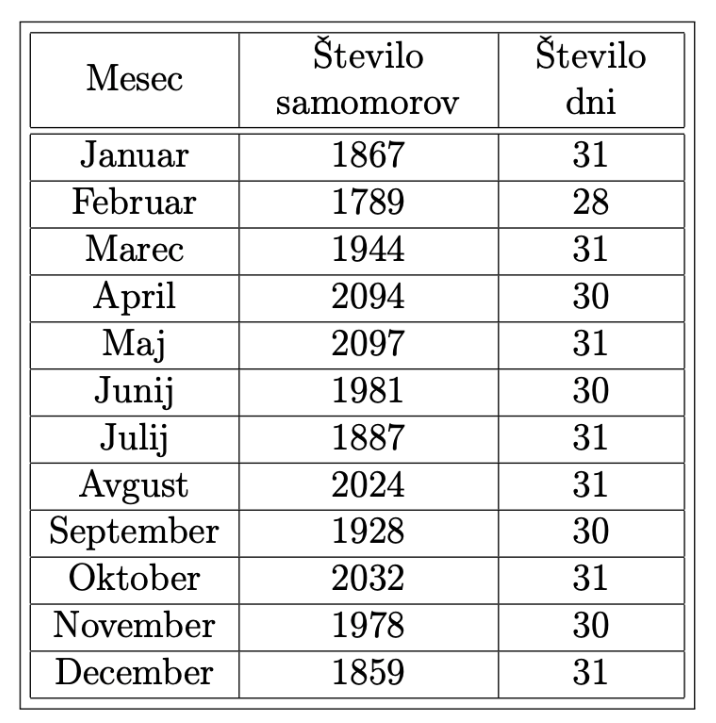
\includegraphics[width=80mm]{samomori.png}
    \caption{Podatki o samomorih}
\end{figure}

\noindent
\textsc{\underline{Primer a}}
\\
Narišemo histogram, pri katerem so širine stolpcev sorazmerne dolžinam mesecev. 
\\
\noindent
\textsc{\underline{Primer b}}
\\
V knjigi \textit{John A. Rice: Mathematical Statistics and Data Analysis} (stran $343$, $344$) preberemo o Pearsonovem $\chi^2$ testu, ki ga bomo uporabili v našem primeru.
\\
Označimo z $1$ mesec januar, z $2$ febaruar in po vrsti naprej do $12$ za december. 
\\
Preveriti želimo predpostavko, da je samomorilnost skozi celo leto konstanta, kar pomeni, da je konstantna za vseh 12 mesecev (razmerje samomorov v posameznem mesecu je torej $\frac{1}{12}$). Naš test bo v tem primeru enak:
$$ H_0 : p_1 = p_2 = \ldots = p_{12} = \frac{1}{12} $$
$$ H_1 : \text{vsaj ena izmed} \  p_1, \ldots, p_{12} \ \text{ni enaka} \ \frac{1}{12} $$
Uporabili bomo Parsonovo $\chi^2$ statistiko:
\begin{align}\label{en:hi}
    \chi^2 = \sum_{i = 1}^{12} \frac{(O_i - E_i)^2}{E_i} \xrightarrow{n \rightarrow \infty} \chi_{m - k - 1}^2, 
\end{align}
kjer je $m = 12$, k število ocenjenih parametrov, kar je v napem primeru $0$. Imamo torej $11$ prostostnih stopenj. $O_i$ je opazovan rezultat, torej podatek, koliko samomorov se v mesecu zgodi.
\\
Iz spodnje tabele (slika iz \textit{John A. Rice: Mathematical Statistics and Data Analysis}) vidimo, da je točka, ki določa zgornjih $5\%$ $\chi^2$ testa z 11 prostostnimi stopnjami enaka $26.76$. To pomeni, da test ovržemo, če $\chi^2 > 26.76$. 
\begin{figure}[ht!]
    \centering
    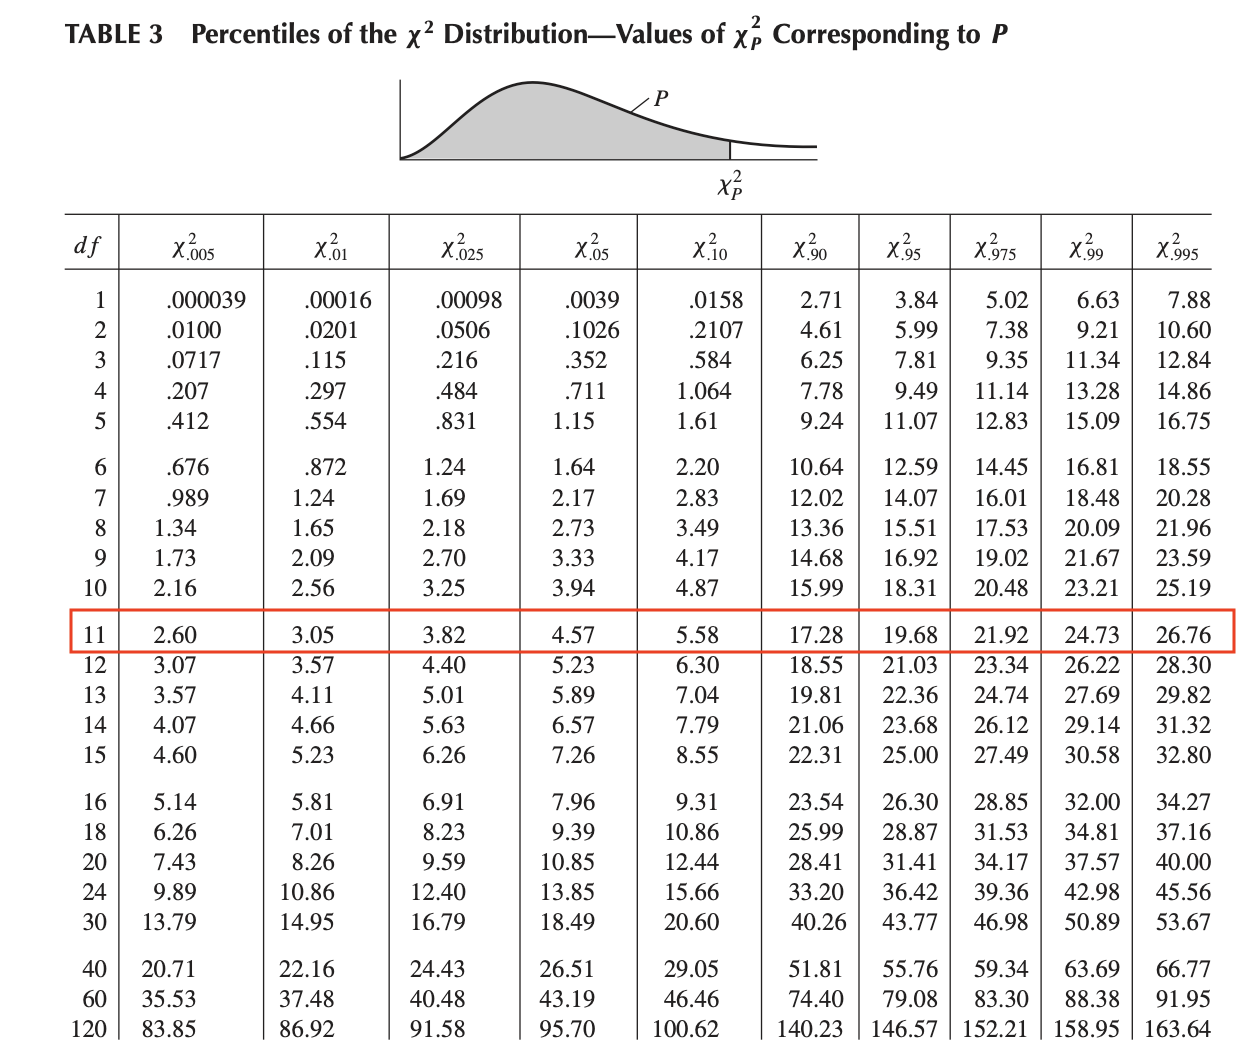
\includegraphics[width=130mm]{hi.png}
    \caption{Hi kvadrat porazdelitev glede na prostostne stopnje.}
\end{figure}

\noindent
Izračunajmo $\chi^2$.
Seštejmo vse samomore v letu in seštevek označimo z $N$. Velja $ N = 1867 + 1789 + \ldots + 1859 = 23480$. Po ničelni hipotezi velja, da je $p_i = \frac{1}{12}, \ \forall i = 1, 2, \ldots, 12$. Velja torej 
$$\text{E}_i =  N \cdot p_i = 1956.67, \ \forall i = 1, 2, \ldots, 12.$$
Za lažji pregled zapišimo podatke za rabo izračuna (\ref{en:hi}) v tabelo:
\\
\begin{table}[h!]
    \begin{center}
        \begin{tabular}{|c|c|c|c|c|c|c|c|c|c|c|c|c|}
            \hline
            \rowcolor[HTML]{FFFFFF} 
            {\color[HTML]{333333} \textbf{$i$}}                                                 & \textbf{1}                   & \textbf{2}                   & \textbf{3}                   & \textbf{4}                   & \textbf{5}                   & \textbf{6}                   & \textbf{7}                   & \textbf{8}                   & \textbf{9}                   & \textbf{10}                  & \textbf{11}                  & \textbf{12} \\ \hline
            \cellcolor[HTML]{FFFFFF}{\color[HTML]{333333} \textbf{$O_i$}}                       & \cellcolor[HTML]{FFFFFF}1867 & \cellcolor[HTML]{FFFFFF}1789 & \cellcolor[HTML]{FFFFFF}1944 & \cellcolor[HTML]{FFFFFF}2094 & \cellcolor[HTML]{FFFFFF}2097 & \cellcolor[HTML]{FFFFFF}1981 & \cellcolor[HTML]{FFFFFF}1887 & \cellcolor[HTML]{FFFFFF}2024 & \cellcolor[HTML]{FFFFFF}1928 & \cellcolor[HTML]{FFFFFF}2032 & \cellcolor[HTML]{FFFFFF}1978 & 1859        \\ \hline
            \cellcolor[HTML]{FFFFFF}{\color[HTML]{333333} \textbf{$\frac{(O_i - E_i)^2}{E_i}$}} & 4.11                         & 14.37                        & 0.08                         & 9.64                         & 10.06                        & 0.30                         & 2.48                         & 2.32                         & 0.42                         & 2.90                         & 0.23                         & 4.88        \\ \hline
        \end{tabular}
    \end{center}
\end{table}

\noindent
Vrednost $\chi^2$ statistike je vsota števil v zadnji vrstici tabele. Velja torej
$$ \chi^2 = 4.11 + 14.37 + \ldots + 4.88 = 51.79 $$
Iz zgornjih sklepov sledi, da $H_0$ zavržemo, saj je $51.79 > 26.76$. Zavrnili smo torej hipotezo, da je razmerje samomorov v posameznih mesecih konstantno.
\\
\\
Če še malo analiziramo podatke v tabeli, vidimo, da k testni statistiki največ prispevajo meseci februar, april in maj, saj imajo glede na druge mesece zelo visoko vrednost. Pri teh treh mesecih se pričakovano število samomorov in dejansko število samomorov za največ razlikujeta.
\\
\begin{figure}[ht!]
    \centering
    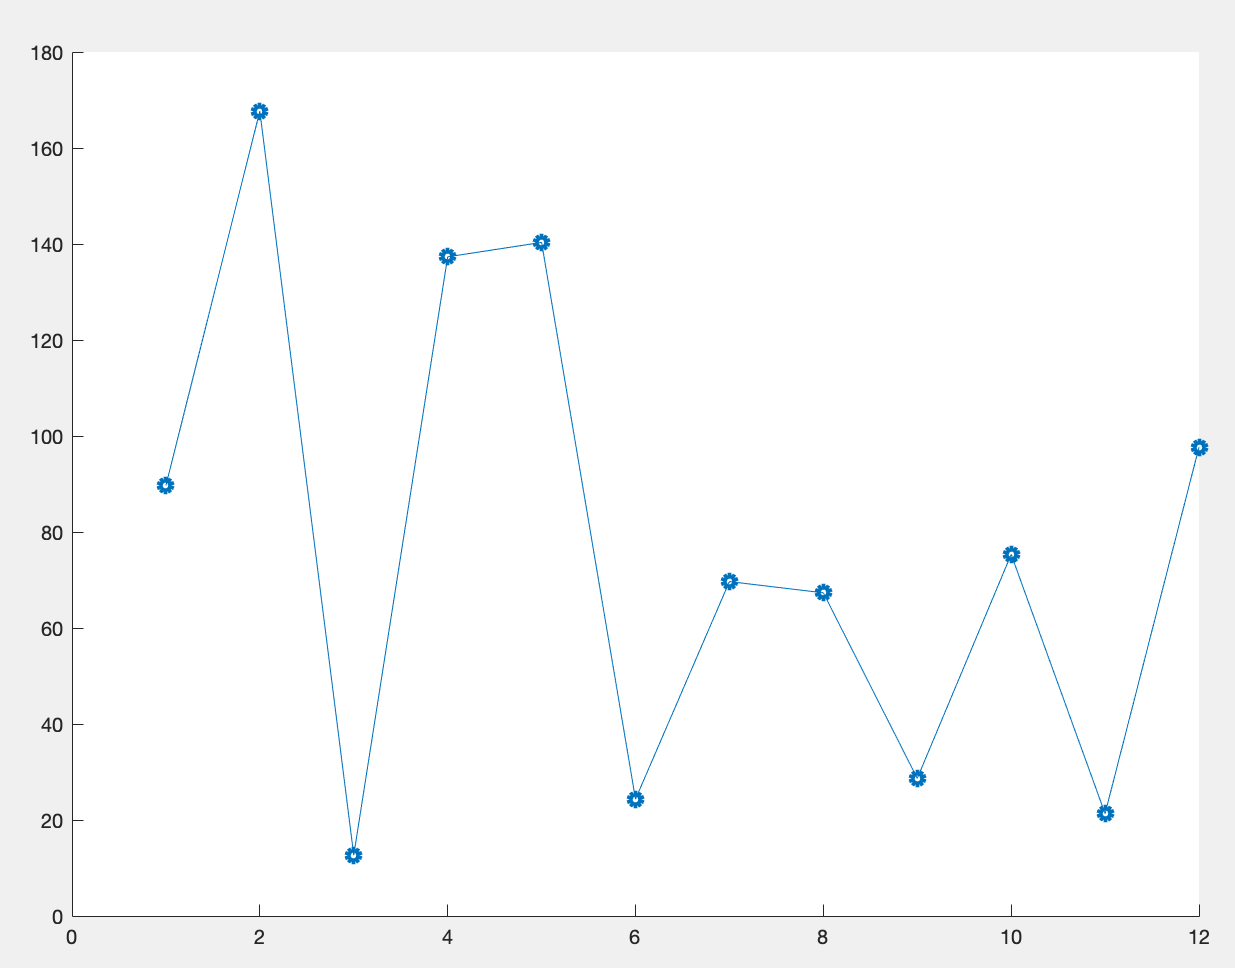
\includegraphics[width=100mm]{razp.png}
    \caption{Absolutne razlike med pričakovanim in dejanskim številom samomorv za posamezni mesec}
\end{figure}

\noindent
Iz grafa ne vidimo nobenega vzorca, ki bi nam lahko kaj povedal o številu samomorov glede na posamezni mesec.
\\
\\
%%%%%%%%%%%%%%%%%%%%%%%%%%%%%%%%%%%%%%%%%%%%%%%%%%%%%%%%%%%%%%
\noindent
\textsc{\large{5. NALOGA}}
\\
\\
$X$ in $Y$ sta slučajni spremenljivki, za kateri velja:
\begin{itemize} 
    \item $\text{E}(X) = \mu_x$,
    \item $\text{E}(Y) = \mu_y$,
    \item $\text{var}(X) = \sigma_x^2$,
    \item $\text{var}(Y) = \sigma_y^2$,
    \item $\text{cov}(X,Y) = \sigma_{x,y}$.
\end{itemize}
Opazimo $X$ in želimo napovedati $Y$. 
\\

\noindent
\textsc{\underline{Primer a}}
\\
Poiščemo napoved, ki je oblike $\hat{Y} = \alpha + \beta \cdot X$, kjer $\alpha$ in $\beta$ izberemo tako, da je srednja kvadratična napaka $\text{E} \left[ \left( Y - \hat{Y} \right) ^2 \right]$ minimalna.
\\
Uporabimo namig 
\begin{align} 
    \text{E} \left[ \left( Y - \hat{Y} \right) ^2 \right] = \left[ \text{E}(Y) - \text{E}(\hat{Y}) \right]^2 + \text{var}(Y - \hat{Y}).
\end{align}
Ker sta oba člena desne strani enačbe večja od $0$, je dovolj, da poiščemo vrednosti $\alpha$ in $\beta$, ki minimizirata ta dva člena -- potem bo najmanjša možna tudi njuna vsota.
\\
Poglejmo si najprej prvi člen enačbe. Vrednost enačbe

\begin{align*}
    \left[ \text{E}(Y) - \text{E}(\hat{Y}) \right]^2 = \left[ \mu_y - \alpha - \beta \mu_x \right] ^2 
\end{align*}
bo najmanjša, ko bo $ \mu_y - \alpha - \beta \cdot \mu_x = 0$. To pa bo res natanko takrat, ko bo $\alpha = \mu_y - \beta \mu_x$. 
\\
Poglejmo si še drugi člen enačbe. Vidimo, da je 

\begin{align*} 
\text{var}(Y-\hat{Y}) &= \text{var}(Y - \alpha - \beta X) = \text{var}(Y - \beta X) = \text{var}(Y) - 2 \beta \text{cov}(X, Y) + \beta^2 \text{var}(X)
\\
&= \sigma_y^2 - 2 \beta \sigma_{x,y} + \beta^2 \sigma_x^2 
\end{align*}
funkcija spremenljivke $\beta$. Za izračun minimuma enačbo najprej odvajamo po $\beta$ in enačimo z $0$.

\begin{align*}
    \frac{\partial}{\partial \beta} (\text{var}(Y - \hat{Y})) = - 2 \sigma_{x,y} + 2 \beta \sigma_x^2 = 0 
\end{align*}
To bo res, ko bo $ \beta = \frac{\sigma_{x,y}}{\sigma_x^2} $.
\\
Vrednosti $\alpha$ in $\beta$, pri katerih bo izraz $\text{E} \left[ \left( Y - \hat{Y}) \right) ^2 \right]$ minimalen, sta
$$ \alpha = \mu_y - \mu_x \frac{\sigma_{x,y}}{\sigma_x^2} \ \ \ \ \ \text{in} \ \ \ \ \ \beta = \frac{\sigma_{x,y}}{\sigma_x^2} $$

\noindent
\textsc{\underline{Primer b}}
\\
Pokažemo, da se pri tako izbranih koeficientih \textit{determinacijski koeficient} (kvadrat korelacijskega koeficienta) izraža v obliki
$$ r_{x,y}^2 = 1 - \frac{\text{var}(Y - \hat{Y})}{\text{var}(Y)}. $$
\\
Spomnimo se najprej formule za \textit{korelacijski koeficient}: 
$$ \text{corr}(X,Y) = \frac{\text{cov}(X,Y)}{\sqrt{\text{var}(X) \text{var}(Y)}} = r_{x,y}. $$
Ker je determinacijski koeficient enak kvadratu korelacije, je enak
$$ r_{x,y}^2 = \frac{\text{cov}(X,Y)^2}{\text{var}(X) \text{var}(Y)}. $$
Želimo torej pokazati
$$ 1 - \frac{\text{var}(Y - \hat{Y})}{\text{var}(Y)} = \frac{\text{cov}(X,Y)^2}{\text{var}(X) \text{var}(Y)}. $$
Če upoštevamo vrednosti $\alpha$ in $\beta$ iz prvega dela naloge, lahko zapišemo
\begin{align*} 
    1 - \frac{\text{var}(Y - \hat{Y})}{\text{var}(Y)} &= \frac{\text{var}(Y) - \text{var}(Y - \hat{Y})}{\text{var}(Y)} = \frac{\sigma_y^2 - \sigma_y^2 + \frac{\sigma_{x,y}^2}{\sigma_x^2}}{\sigma_y^2} 
    \\
    &= \frac{\sigma_{x,y}^2}{\sigma_x^2 \sigma_y^2} = \frac{\text{cov}(X,Y)^2}{\text{var}(X) \text{var}(Y)} = r_{x,y}^2. 
\end{align*}
Pokazali smo, da je determinacijski koeficient res enak $1 - \frac{\text{var}(Y - \hat{Y})}{\text{var}(Y)}$.
%%%%%%%%%%%%%%%%%%%%%%%%%%%%%%%%%%%%%%%%%%%%%%%%%%%%%%%%%%%%%%
\end{document}
